\clearpage
\item \points{40} {\bf Linear Classifiers (logistic regression and GDA)}

In this problem, we cover two probabilistic linear classifiers we have
covered in class so far. First, a discriminative linear classifier: logistic
regression. Second, a generative linear classifier: Gaussian discriminant
analysis (GDA). Both the algorithms find a linear decision boundary that
separates the data into two classes, but make different assumptions. Our goal
in this problem is to get a deeper understanding of the similarities and
differences (and, strengths and weaknesses) of these two algorithms.

For this problem, we will consider two datasets, provided in the following
files:
\begin{enumerate}[label=\roman*.]
	\item \url{data/ds1_{train,valid}.csv}
	\item \url{data/ds2_{train,valid}.csv}
\end{enumerate}
Each file contains $m$ examples, one example $(x^{(i)}, y^{(i)})$ per row.
In particular, the $i$-th row contains columns $x^{(i)}_0\in\Re$,
$x^{(i)}_1\in\Re$, and $y^{(i)}\in\{0, 1\}$. In the subproblems that follow, we
will investigate using logistic regression and Gaussian discriminant analysis
(GDA) to perform binary classification on these two datasets.

\begin{enumerate}
	\item \subquestionpoints{10}
In lecture we saw the average empirical loss for logistic regression:
\begin{equation*}
	J(\theta)
	= -\frac{1}{m} \sum_{i=1}^m y^{(i)}\log(h_{\theta}(x^{(i)}))
		+  (1 - y^{(i)})\log(1 - h_{\theta}(x^{(i)})),
\end{equation*}
where $y^{(i)} \in \{0, 1\}$, $h_\theta(x) = g(\theta^T x)$ and
$g(z) = 1 / (1 + e^{-z})$.

Find the Hessian $H$ of this function, and show that for any vector $z$, it
holds true that
%
\begin{equation*}
    z^T H z \ge 0.
\end{equation*}
%
{\bf Hint:} You may want to start by showing that
$\sum_i\sum_j z_i x_i x_j z_j = (x^Tz)^2 \geq 0$. Recall also that
$g'(z) = g(z)(1-g(z))$.

{\bf Remark:} This is one of the standard ways of showing that the matrix $H$
is positive semi-definite, written ``$H \succeq 0$.''  This implies that $J$ is
convex, and has no local minima other than the global one. If you have some
other way of showing $H \succeq 0$, you're also welcome to use your method
instead of the one above.

\ifnum\solutions=1 {
  \begin{answer}\\
$\sum_{i=1}^{n}\sum_{j=i}^{n}z_ix_ix_jz_j=x_i^2+2x_1z_1x_2z_2+\dots+2x_1z_1x_nz_n+x_2^2z_2^2+2x_2z_2x_3z_3+\dots+x_n^2z_n^2$\\
$(x^Tz)^2=x_i^2+2x_1z_1x_2z_2+\dots+2x_1z_1x_nz_n+x_2^2z_2^2+2x_2z_2x_3z_3+\dots+x_n^2z_n^2$\\
$\therefore \sum_{i=1}^{n}\sum_{j=i}^{n}z_ix_ix_jz_j=(x^Tz)^2 \geq 0$\\
$J(\theta)=-\frac{1}{m}\sum_{i=1}^{m}\left[ y^{(i)}log(g(\theta^T z^{(i)})) + (1-y^{(i)})log(1-g(\theta^T z^{(i)})) \right]$\\
$=\frac{1}{m}\sum_{i=1}^{m} - \left[ y^{(i)}log(g(\theta^T x^{(i)})) + (1-y^{(i)})log(1-g(\theta^T x^{(i)})) \right]$\\
We can ignore the $\frac{1}{m}$ in the derivative since it is a constant and doesnt change the calculations\\
$\therefore \frac{\partial J}{\partial \theta_j}=-(y \frac{1}{g(\theta^T x)}g(\theta^T x)(1-g(\theta^T x))x_j + (1-y)\frac{1}{1-g(\theta^T x)}-g(\theta^T x)(1-g(\theta^T x))x_j)$
$=-(yx_j-yx_jg(\theta^T x)-g(\theta^T x)x_j +yx_jg(\theta^T x))=\frac{1}{m} g(\theta^T x)x_j -yx_j$\\

$\therefore \frac{\partial J^2}{\partial \theta_1^2}=g(\theta^T x)(1-g(\theta^T x))x_1^2$, $\frac{\partial J^2}{\partial \theta_1\theta_2}=g(\theta^T x)(1-g(\theta^T x))x_1x_2$ and so on...\\
$\therefore H=$
\[
\begin{bmatrix}
g(\theta^T x)(1-g(\theta^T x))x_1^2 & g(\theta^T x)(1-g(\theta^T x))x_1x_2 & \dots & g(\theta^T x)(1-g(\theta^T x))x_1x_n \\
g(\theta^T x)(1-g(\theta^T x))x_1x_2 & g(\theta^T x)(1-g(\theta^T x))x_2^2 & \dots & g(\theta^T x)(1-g(\theta^T x))x_2x_n \\
\vdots & \vdots & \vdots  & \vdots \\
g(\theta^T x)(1-g(\theta^T x))x_1x_n & g(\theta^T x)(1-g(\theta^T x))z_2x_n & \dots & g(\theta^T x)(1-g(\theta^T x))x_n^2 \\
\end{bmatrix}
\]=$g(\theta^T x)(1-g(\theta^T x))$
\[
\begin{bmatrix}
x_1^2 & x_1x_2 & \dots & x_1x_n \\
x_1x_2 & x_2^2 & \dots & x_2x_n \\
\vdots & \vdots & \vdots  & \vdots \\
x_1x_n & z_2x_n & \dots & x_n^2 \\
\end{bmatrix}
\]\\
but $0 \leq g(\theta^T x) \leq 1$ since its the sigmoid function. Also $0 \leq (1-g(\theta^T x)) \leq1$\\
$\therefore z^THz=g(\theta^T x)(1-g(\theta^T x))(z_1^2x_1^2+2z_1x_1x_2z_2+\dots+z_n^2x_n^2)=g(\theta^T x)(1-g(\theta^T x))(x^Tz)^2$\\
we already showed $(x^Tz)^2 \geq 0$\\
$\therefore z^THz \geq 0$
\end{answer}
} \fi

	\clearpage
\item \subquestionpoints{5} \textbf{Coding problem.}
Follow the instructions in \texttt{src/p01b\_logreg.py} to train a
logistic regression classifier using Newton's Method.
Starting with $\theta = \vec{0}$, run Newton's Method until the updates to
$\theta$ are small: Specifically,  train until the first iteration $k$ such
that $\|\theta_{k} - \theta_{k-1}\|_1 < \epsilon$, where
$\epsilon = 1\times 10^{-5}$. Make sure to write your model's predictions to
the file specified in the code.

\ifnum\solutions=1 {
  \begin{answer}
\end{answer}

} \fi

	\clearpage
\item \subquestionpoints{5}
Recall that in GDA we model the joint distribution of $(x, y)$ by the following
equations:
%
\begin{eqnarray*}
	p(y) &=& \begin{cases}
	\phi & \mbox{if~} y = 1 \\
	1 - \phi & \mbox{if~} y = 0 \end{cases} \\
	p(x | y=0) &=& \frac{1}{(2\pi)^{n/2} |\Sigma|^{1/2}}
		\exp\left(-\frac{1}{2}(x-\mu_{0})^T \Sigma^{-1} (x-\mu_{0})\right) \\
	p(x | y=1) &=& \frac{1}{(2\pi)^{n/2} |\Sigma|^{1/2}}
		\exp\left(-\frac{1}{2}(x-\mu_1)^T \Sigma^{-1} (x-\mu_1) \right),
\end{eqnarray*}
%
where $\phi$, $\mu_0$, $\mu_1$, and $\Sigma$ are the parameters of our model.

Suppose we have already fit $\phi$, $\mu_0$, $\mu_1$, and $\Sigma$, and now
want to predict $y$ given a new point $x$. To show that GDA results in a
classifier that has a linear decision boundary, show the posterior distribution
can be written as
%
\begin{equation*}
	p(y = 1\mid x; \phi, \mu_0, \mu_1, \Sigma)
	= \frac{1}{1 + \exp(-(\theta^T x + \theta_0))},
\end{equation*}
%
where $\theta\in\Re^n$ and $\theta_{0}\in\Re$ are appropriate functions of
$\phi$, $\Sigma$, $\mu_0$, and $\mu_1$.

\ifnum\solutions=1{
  \begin{answer}
\end{answer}

}\fi

	\clearpage
\item \subquestionpoints{7} For this part of the problem only, you may
  assume $n$ (the dimension of $x$) is 1, so that $\Sigma = [\sigma^2]$ is
  just a real number, and likewise the determinant of $\Sigma$ is given by
  $|\Sigma| = \sigma^2$.  Given the dataset, we claim that the maximum
  likelihood estimates of the parameters are given by
  \begin{eqnarray*}
    \phi &=& \frac{1}{m} \sum_{i=1}^m 1\{y^{(i)} = 1\} \\
\mu_{0} &=& \frac{\sum_{i=1}^m 1\{y^{(i)} = {0}\} x^{(i)}}{\sum_{i=1}^m
1\{y^{(i)} = {0}\}} \\
\mu_1 &=& \frac{\sum_{i=1}^m 1\{y^{(i)} = 1\} x^{(i)}}{\sum_{i=1}^m 1\{y^{(i)}
= 1\}} \\
\Sigma &=& \frac{1}{m} \sum_{i=1}^m (x^{(i)} - \mu_{y^{(i)}}) (x^{(i)} -
\mu_{y^{(i)}})^T
  \end{eqnarray*}
  The log-likelihood of the data is
  \begin{eqnarray*}
\ell(\phi, \mu_{0}, \mu_1, \Sigma) &=& \log \prod_{i=1}^m p(x^{(i)} , y^{(i)};
\phi, \mu_{0}, \mu_1, \Sigma) \\
&=& \log \prod_{i=1}^m p(x^{(i)} | y^{(i)}; \mu_{0}, \mu_1, \Sigma) p(y^{(i)};
\phi).
  \end{eqnarray*}
By maximizing $\ell$ with respect to the four parameters,
prove that the maximum likelihood estimates of $\phi$, $\mu_{0}, \mu_1$, and
$\Sigma$ are indeed as given in the formulas above.  (You may assume that there
is at least one positive and one negative example, so that the denominators in
the definitions of $\mu_{0}$ and $\mu_1$ above are non-zero.)

\ifnum\solutions=1 {
  \begin{answer}\\
We know that\\
$p(y;\phi)$
$\begin{cases}
\phi $ if $y=1\\
1-\phi$ if $y=0\\
\end{cases}$\\
and\\
$p(x^{(i)}|y^{(i)}=0;\mu_0,\mu_1,\sigma)=\frac{1}{(2 \pi \sigma^2)^{1/2}}e^{-\frac{1}{2 \sigma^2}(x^{(i)}-\mu_0)^2}$\\
$p(x^{(i)}|y^{(i)}=1;\mu_0,\mu_1,\sigma)=\frac{1}{(2 \pi \sigma^2)^{1/2}}e^{-\frac{1}{2 \sigma^2}(x^{(i)}-\mu_1)^2}$\\
$l=log\prod_{i=1}^{m}p(x^{(i)}|y^{(i)};\mu_0,\mu_1,\sigma)p(y;\phi)=\sum_{i=1}^{m}log(p(x^{(i)}|y^{(i)};\mu_0,\mu_1,\sigma))+\sum_{i=1}^{m}log(p(y;\phi))$\\
$=\sum_{i=1}^{m}[log{1}-\frac{1}{2}log(2 \pi) -\frac{1}{2}log(\sigma^2)-\frac{1}{2 \sigma^2}(x^{(i)}-\mu_{y^{(i)}})^2]+\sum_{i=1}^{m}y^{(i)}log \phi + (1-y^{(i)})log(1-\phi)$\\\\
$\therefore \frac{\partial l}{\partial \phi}=\sum_{i=1}^{m}[\frac{y^{(i)}}{\phi}+\frac{1-y^{(i)}}{1-\phi}]=\frac{\sum_{i=1}^{m}1 \lbrace y^{(i)}=1 \rbrace }{\phi}+\frac{m-\sum_{i=1}^{m}1 \lbrace y^{(i)}=1 \rbrace}{1-\phi}=\frac{m \phi -\sum_{i=1}^{m}1 \lbrace y^{(i)}=1 \rbrace}{\phi (1-\phi)}$\\
To naximize the log likelihood (and therefore the likelihood) we set the derivative to zero. We also know that we have at least 1 positive and negative example (each) so $\phi > 0$ and $1-\phi > 0$. Therefore we solve for the numerator=0\\
$\therefore \frac{m \phi -\sum_{i=1}^{m}1 \lbrace y^{(i)}=1 \rbrace}{\phi (1-\phi)} \implies \phi=\frac{\sum_{i=1}^{m}1 \lbrace y^{(i)}=1 \rbrace}{m}$\\
Similarly\\
$\frac{\partial l}{\partial \mu_0}=\sum_{i;y^{(i)}=0}-\frac{1}{2 \sigma^2} \cdot 2 (x^{(i)}-\mu_0) \cdot -1=\frac{1}{\sigma^2}\sum_{i;y^{(i)}=0}(x^{(i)}-\mu_0)$\\
Again, solving for this derivative=0 (note that $\sigma^2>0$) we have\\
$\sum_{i;y^{(i)}=0}x^{(i)}=\sum_{i;y^{(i)}=0}\mu_0$\\
but $\sum_{i;y^{(i)}=0}x^{(i)}=\sum_{i=1}^{m}1 \lbrace y^{(i)}=0 \rbrace x^{(i)}$ and $\sum_{i;y^{(i)}=0}\mu_0=\sum_{i=1}^{m}1 \lbrace y^{(i)}=0 \rbrace \mu_0$\\
$\therefore \mu_0=\frac{\sum_{i=1}^{m}1 \lbrace y^{(i)}=0 \rbrace x^{(i)}}{\sum_{i=1}^{m}1 \lbrace y^{(i)}=0 \rbrace}$\\
Similarly $\frac{\partial l}{\partial \mu_1}\sum_{i;y^{(i)}=1}=-\frac{1}{2 \sigma^2} \cdot 2 (x^{(i)}-\mu_1) \cdot -1=\frac{1}{\sigma^2}\sum_{i;y^{(i)}=1}(x^{(i)}-\mu_1)$\\
Again, solving for zero we have $\sum_{i;y^{(i)}=1}x^{(i)}=\sum_{i;y^{(i)}=1}\mu_0 \implies \mu_1=\frac{\sum_{i=1}^{m}1 \lbrace y^{(i)}=1 \rbrace x^{(i)}}{\sum_{i=1}^{m}1 \lbrace y^{(i)}=1 \rbrace}$\\
Finally, $\frac{\partial l}{\partial \sum}=\sum_{i=1}^{m}-\frac{1}{2}\frac{1}{\sum}+\frac{1}{2}(x^{(i)}-\mu_{y^{(i)}})^2 \cdot -\frac{1}{\sum^2}$\\
Solving for this =0 we have\\
$\frac{1}{2 \sum^2}\sum_{i=1}^{m} [(x^{(i)}-\mu_{y^{(i)}})^2 -\sum] \implies \sum_{i=1}^{m} (x^{(i)}-\mu_{y^{(i)}})^2 - m \sum=0 $\\
$\implies \sum=\frac{1}{m}\sum_{i=1}^{m} (x^{(i)}-\mu_{y^{(i)}})^2=\frac{1}{m}\sum_{i=1}^{m} (x^{(i)}-\mu_{y^{(i)}})(x^{(i)}-\mu_{y^{(i)}})^T$\\
\end{answer}

} \fi

	\clearpage
\item \subquestionpoints{3} \textbf{Coding problem.}
In \texttt{src/p01e\_gda.py}, fill in the code to
calculate $\phi$, $\mu_{0}$, $\mu_{1}$, and $\Sigma$, use these parameters
to derive $\theta$, and use the resulting GDA model to make predictions on the
validation set.

\ifnum\solutions=1 {
  \begin{answer}
\end{answer}

} \fi

	\clearpage
\item \subquestionpoints{5}
For Dataset 1, create a plot of the validation set with $x_1$ on the horizontal
axis, and $x_2$ on the vertical axis. To visualize the two classes, use a
different symbol for examples $x^{(i)}$ with $y^{(i)} = 0$ than for those with
$y^{(i)} = 1$. On the same figure, plot the decision boundary found by logistic
regression in part (b). Make an identical plot with the decision boundary found
by GDA in part (e).

\ifnum\solutions=1 {
\begin{answer}\\
\begin{figure}
  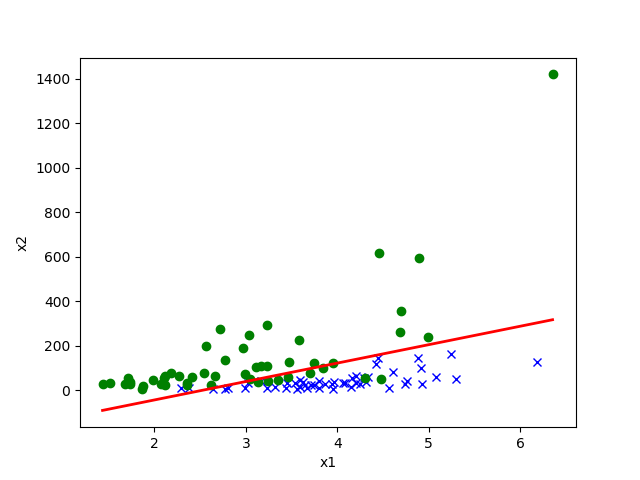
\includegraphics[width=\linewidth]{p01b_pred_1_eval.png}
  \caption{Dateset 1 prediction on EVAL set using LogisticRegression}
  \label{fig:Dateset 1 prediction on EVAL set using LogisticRegression}
\end{figure}\\
\begin{figure}
  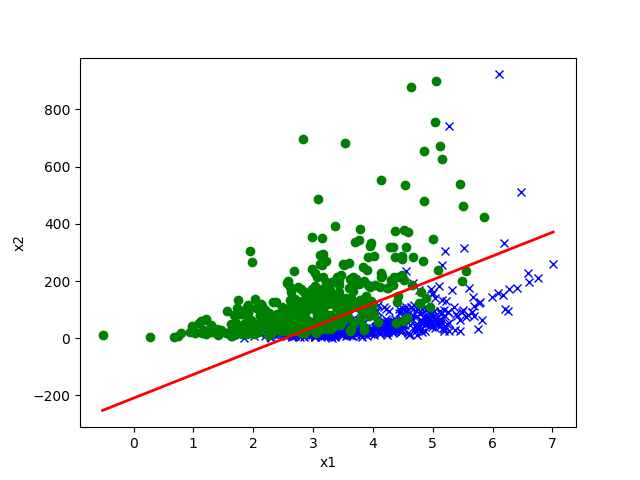
\includegraphics[width=\linewidth]{p01b_pred_1_train.png}
  \caption{Dateset 1 prediction on TRAIN set using LogisticRegression}
  \label{fig:Dateset 1 prediction on TRAIN set using LogisticRegression}
\end{figure}\\
\begin{figure}
  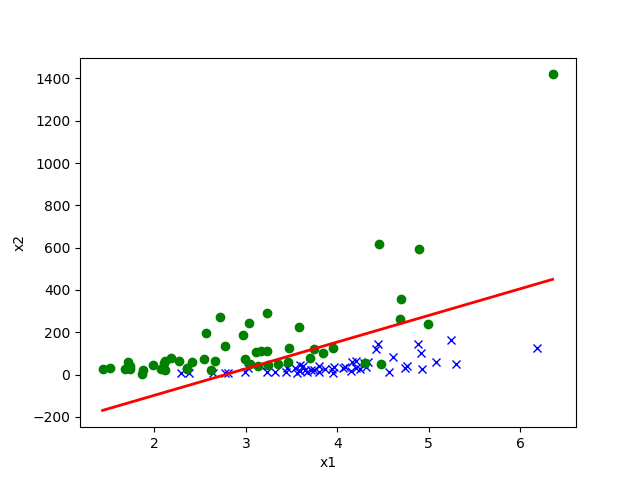
\includegraphics[width=\linewidth]{p01e_pred_1_eval.png}
  \caption{Dateset 1 prediction on EVAL set using GDA}
  \label{fig:Dateset 1 prediction on EVAL set using GDA}
\end{figure}\\
\begin{figure}
  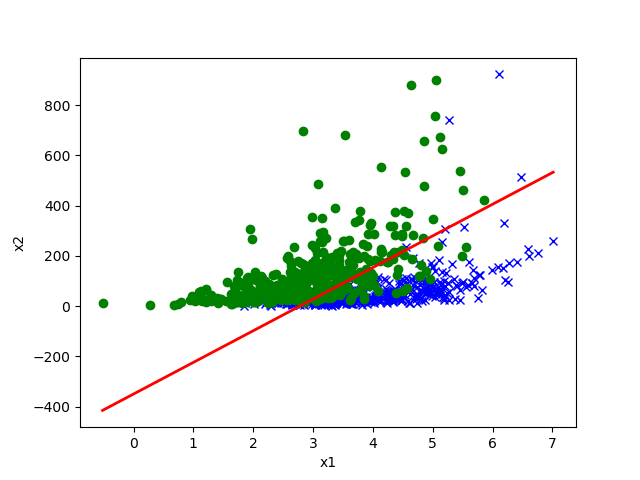
\includegraphics[width=\linewidth]{p01e_pred_1_train.png}
  \caption{Dateset 1 prediction on TRAIN set using GDA}
  \label{fig:Dateset 1 prediction on TRAIN set using GDA}
\end{figure}\\
\end{answer}

} \fi

	\clearpage
\item \subquestionpoints{5}
Repeat the steps in part (f) for Dataset 2. On which dataset does GDA seem to
perform worse than logistic regression? Why might this be the case?

\ifnum\solutions=1{
  \begin{answer}
\begin{figure}
  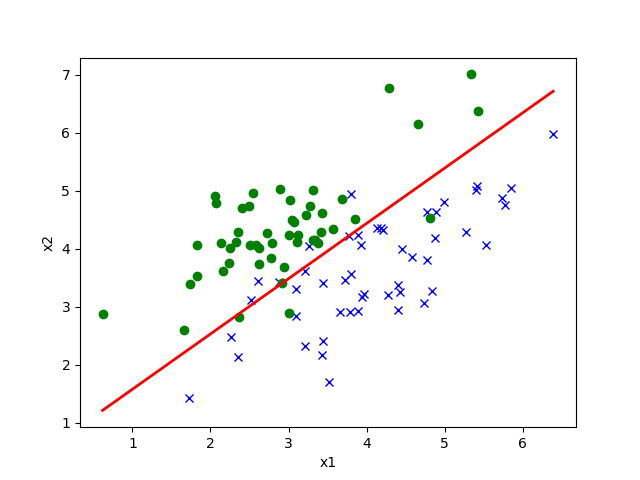
\includegraphics[width=\linewidth]{p01b_pred_2_eval.png}
  \caption{Dateset 2 prediction on EVAL set using LogisticRegression}
  \label{fig:Dateset 2 prediction on EVAL set using LogisticRegression}
\end{figure}\\
\begin{figure}
  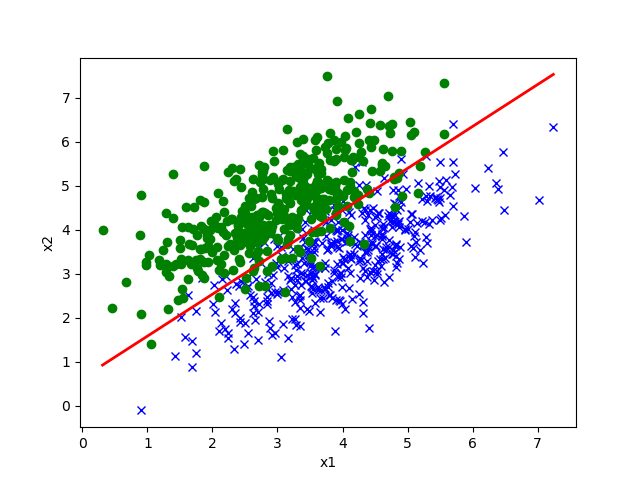
\includegraphics[width=\linewidth]{p01b_pred_2_train.png}
  \caption{Dateset 2 prediction on TRAIN set using LogisticRegression}
  \label{fig:Dateset 2 prediction on TRAIN set using LogisticRegression}
\end{figure}\\
\begin{figure}
  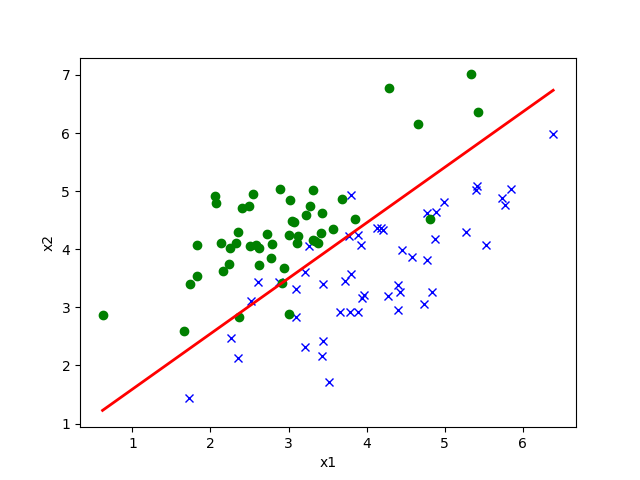
\includegraphics[width=\linewidth]{p01e_pred_2_eval.png}
  \caption{Dateset 2 prediction on EVAL set using GDA}
  \label{fig:Dateset 2 prediction on EVAL set using GDA}
\end{figure}\\
\begin{figure}
  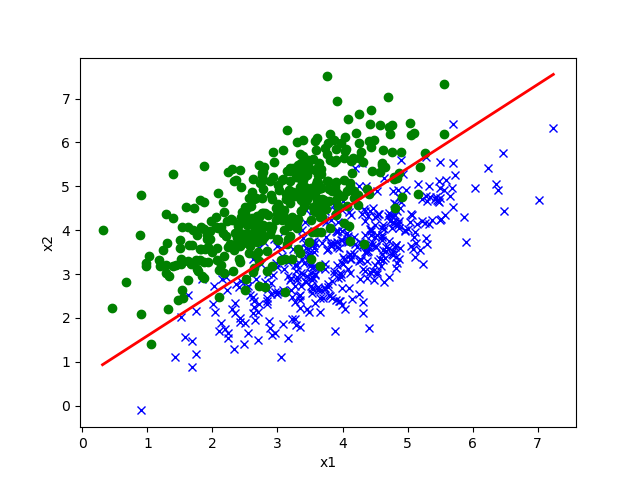
\includegraphics[width=\linewidth]{p01e_pred_2_train.png}
  \caption{Dateset 2 prediction on TRAIN set using GDA}
  \label{fig:Dateset 2 prediction on TRAIN set using GDA}
\end{figure}\\
GDA does worse on the first dataset. This is the case because we have some points that are outliers that are skewing the calculations of $\mu_0, \mu_1$ and $\sigma$. 
\end{answer}

}\fi

	\clearpage
\item \points{3 extra credit} For the dataset where GDA performed worse in
parts (f) and (g), can you find a transformation of the $x^{(i)}$'s such
that GDA performs significantly better? What is this transformation?

\ifnum\solutions=1{
  \begin{answer}\\
If we transform $x^{(i)}$ to $log(x^{(i)})$ we would get significantly better performance.\\
\end{answer}

}\fi

\end{enumerate}
